\documentclass[10pt,a4paper]{article}
\usepackage[utf8]{inputenc}
\usepackage[spanish]{babel}
\usepackage{amsmath}
\usepackage{amsfonts}
\usepackage{amssymb}
\usepackage{graphicx}
\usepackage{multicol}
\usepackage{titling}
\usepackage{titlesec}
\usepackage{array}
\usepackage{bm}
\usepackage{afterpage}
\usepackage{float}
\usepackage{graphicx}
\usepackage{epstopdf}
\usepackage{longtable}
\usepackage{xcolor}
\usepackage{epigraph}
\setlength\epigraphwidth{1.5\textwidth}
\usepackage{subfigure}
\usepackage{anyfontsize}
\usepackage[left=2cm,right=2cm,top=2cm,bottom=2cm]{geometry}
\usepackage[colorlinks=true,
            linkcolor=blue,
            citecolor=blue,
            urlcolor=blue]{hyperref}

\begin{document}
\author{Estévez Santiago\\
		Lozada Jhonny\\
		Maya Vicente} % CAMBIAR A AUTORES
\title{MATERIA OPTATIVA II\\ % TITULO  \\ ES ENTER
PROYECTO FINAL PRIMER PARCIAL}
\maketitle  
\section{Introducción} % nuevas secciones
\begin{multicols}{2} % texto en 2 colomnas
El machine learning, en español aprendizaje  es un sub-campo de las ciencias computacionales con varias aplicaciones a diferentes campos de la ingeniería.\\ 
Lo que se desarrollo a continuación es un programa el cual puede clasificar diferentes objetos a través de medidas, de diferentes parámetros que se encuentran almacenados en una base de datos, ademas, selecciona y filtra datos de la base de datos la cual esta guardada una matriz, la cual hace que se los datos queden reducidos a los mejores y de esta manera ahorrar recursos y mejorar el rendimiento de nuestro microprocesador Arduino Mega. \\
El sistema funciona con una matriz de [120][5] la cual es nuestra base de datos mas grande, el programa selecciona los mejores datos a partir de donas, las cuales están ubicadas en medio de  los valores y se mueva al rededor de toda la matriz, buscando el mejor centro para la obtención de datos a futuro de una mejor matriz sin muchos valores, de esta manera se automatiza el ingreso de datos.\\

\end{multicols} %termina texto en columnas
\section{Diseño del Sistema}
\subsection{Diagrama de Flujo y Diagrama de Bloques KNN}
Diagrama de flujo realizado para KNN y CNN unificado
\begin{figure}[H]
\caption{Diagrama de flujo KNN y CNN} % ingresa nombre de la figura (caption)
\centering
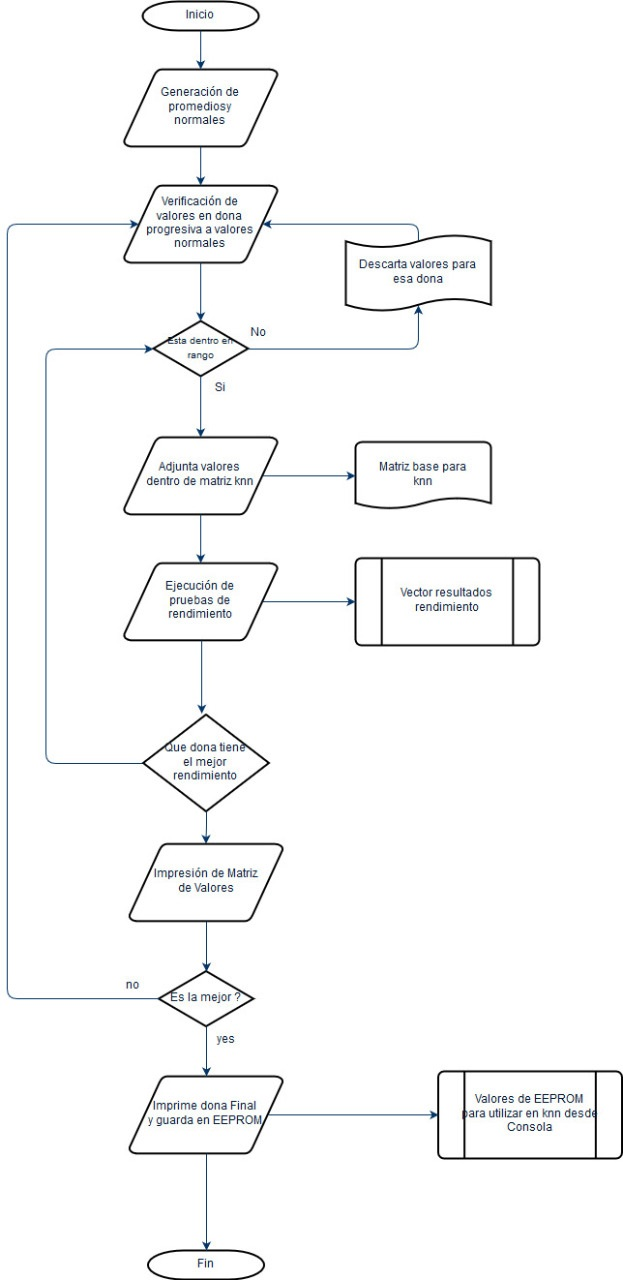
\includegraphics[scale=0.6]{Flujo.jpg} % cambie el valor de la escala entre 0.1-1 para el tamano de la misma
\end{figure}\\ %termina figura y envia enter


\\
Lo principal que se debe tener es la base de datos en este caso esta compuesta de [120][5], de la cual para obtener sus centroides, debemos primero sacar los promedios de cada columna de datos con excepción de la columna de etiqueta, una vez tenemos el promedio se prosigue con las distancias con la fórmula previamente vista y sacamos el valor máximo del grupo de datos, con estos se los procede a normalizar  los valores y por último se obtiene los centroides, estos se los realiza por el método de donas, para este caso se ha realizado que éstas donas empiecen en un rango de 0-0,1 y así sucesivamente ir aumentando 0,1 cada rango, de todo el grupo de datos que llegamos a obtener realizamos la mejor matriz.\\
Para obtener la mejor matriz se aplica KNN a cada una de las matrices generadas con las donas, para saber cuál es la mejor debemos tener en cuenta la eficiencia que aportan cada una de ellas, una vez el programa entiende los cálculos obtiene la mejor matriz y todo esto se realiza de manera autónoma.\\
Ahora finalmente al ingresar un valor de prueba si este es erróneo a la base S y en caso de ser correcto va a la matriz D.
\\

Diagrama de Bloques del sistema KNN
\begin{figure}[H]
\caption{Diagrama de bloques KNN} % ingresa nombre de la figura (caption)
\centering
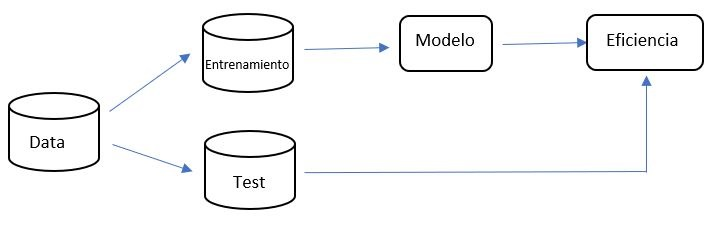
\includegraphics[scale=0.8]{dbknn.png}
\end{figure}
\\
Para realizar KNN lo primero que debemos tener son nuestros datos divididos en dos base de datos, la primera será la base de entrenamiento y la segunda la base de test o de prueba, pero con la que se trabaja es con la matriz de entrenamiento en donde realizando un modelo de donas obtenemos los centroides para generar la mejor matriz de referencia, al tratarse del algoritmo del vecino más cercano nosotros podemos escoger cuántos vecinos necesitamos, en nuestro caso serán 3 vecinos.

\section{Desarrollo}
\subsection{Simulación}
Simulacion de KNN y CNN 
\begin{figure}[H]
\caption{Simulacion en proteus}
\centering
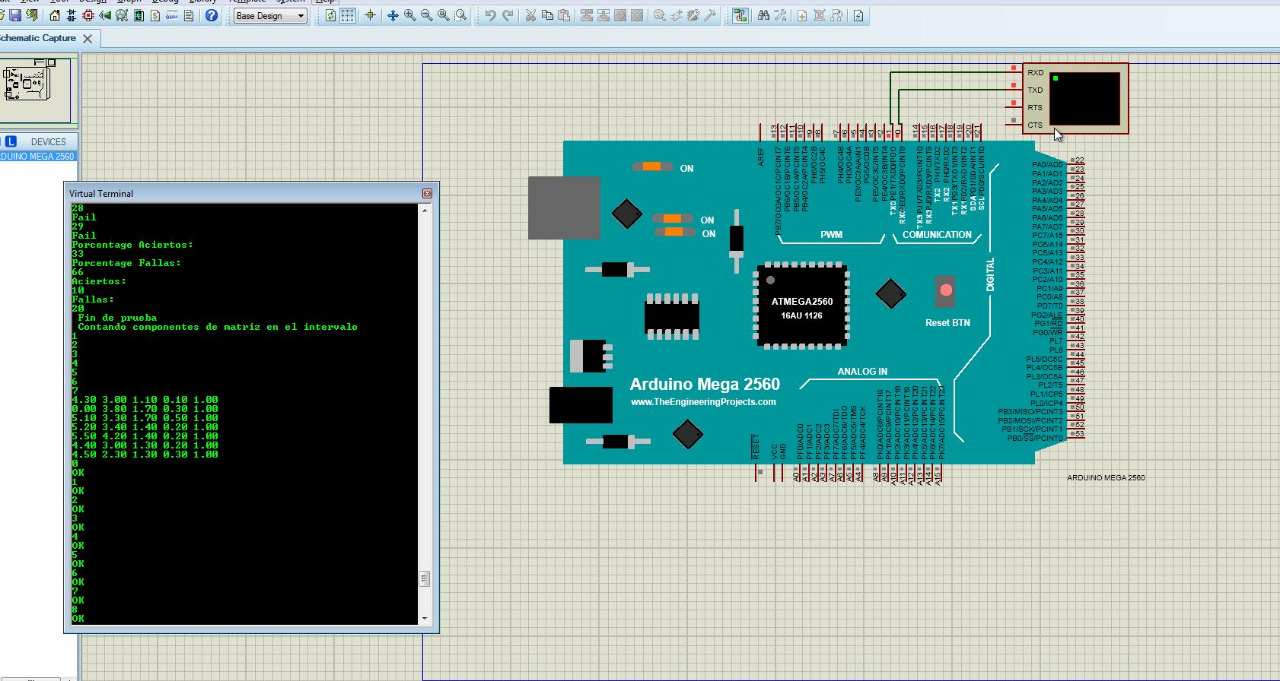
\includegraphics[scale=0.5]{sim.png}
\end{figure} 


\section{Análisis de Resultados}
El sistema Funciona de tal manera que al ejecutarlo recorre toda la matriz original en búsqueda de los mejores datos para generar una nueva matriz y de esta manera cree otra la cual será la adecuada con el fin de ser mas exacta y ocupe menos recursos.\\

A continuación se muestra todo el código de programación el cual se encuentra comentado y se explica por si solo. 
\begin{figure}[H]
\caption{Código Parte 1}
\centering
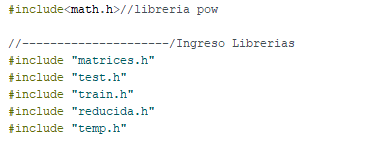
\includegraphics[scale=0.9]{c1.png}
\end{figure}  

\begin{figure}[H]
\caption{Código Parte 2}
\centering
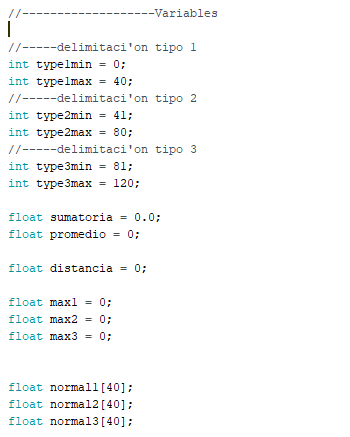
\includegraphics[scale=0.9]{c2.png}
\end{figure}

\begin{figure}[H]
\caption{Código Parte 3}
\centering
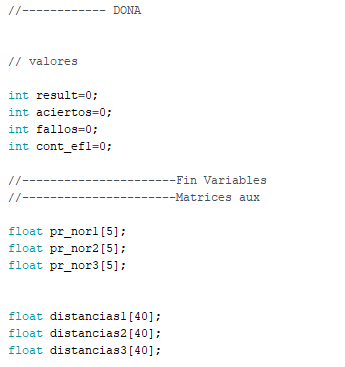
\includegraphics[scale=0.9]{c3.png}
\end{figure}

\begin{figure}[H]
\caption{Código Parte 4}
\centering
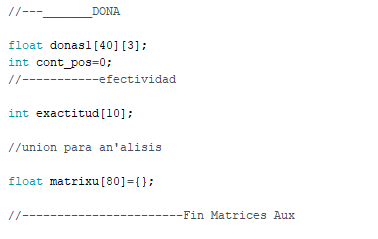
\includegraphics[scale=0.9]{c4.png}
\end{figure}

\begin{figure}[H]
\caption{Código Parte 5}
\centering
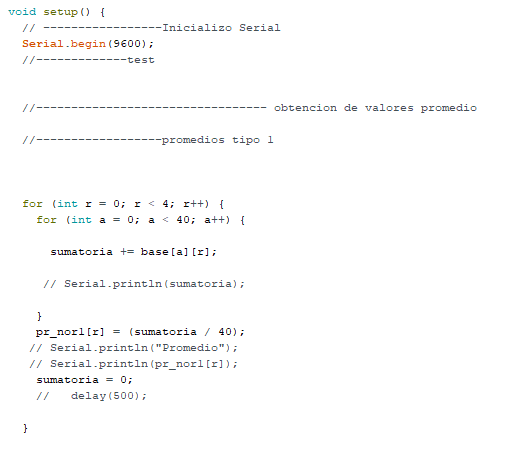
\includegraphics[scale=0.9]{c5.png}
\end{figure}

\begin{figure}[H]
\caption{Código Parte 6}
\centering
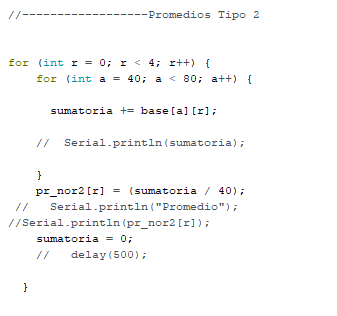
\includegraphics[scale=0.9]{c6.png}
\end{figure}

\begin{figure}[H]
\caption{Código Parte 7}
\centering
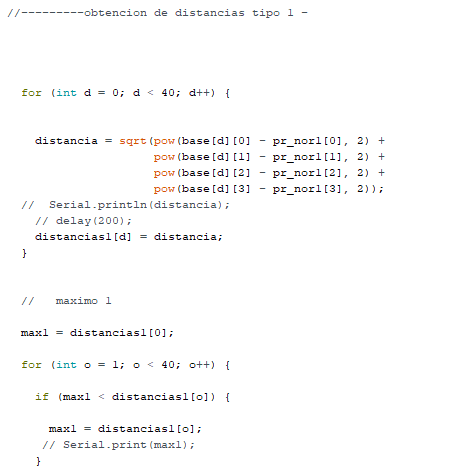
\includegraphics[scale=0.9]{c7.png}
\end{figure}

\begin{figure}[H]
\caption{Código Parte 8}
\centering
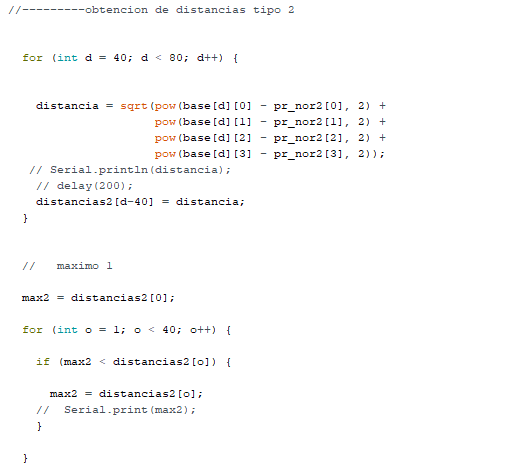
\includegraphics[scale=0.9]{c8.png}
\end{figure}

\begin{figure}[H]
\caption{Código Parte 9}
\centering
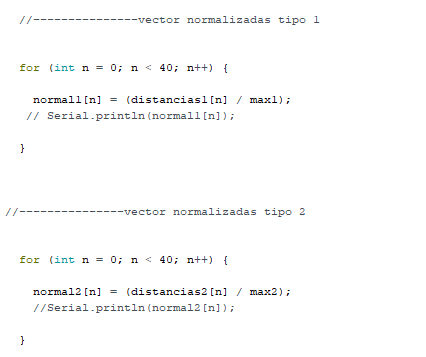
\includegraphics[scale=0.9]{c9.png}
\end{figure}

\begin{figure}[H]
\caption{Código Parte 10}
\centering
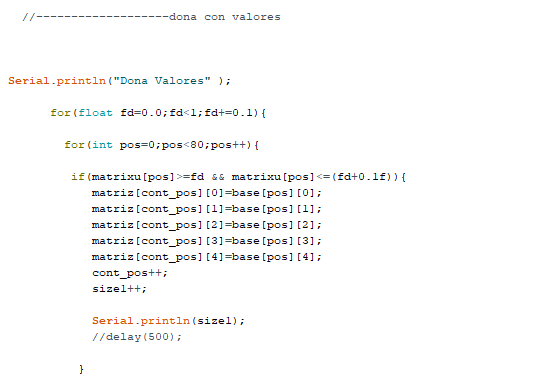
\includegraphics[scale=0.9]{c10.png}
\end{figure}

\begin{figure}[H]
\caption{Código Parte 11}
\centering
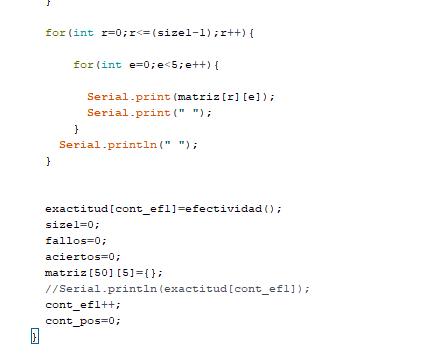
\includegraphics[scale=0.9]{c11.png}
\end{figure}

\begin{figure}[H]
\caption{Código Parte 12}
\centering
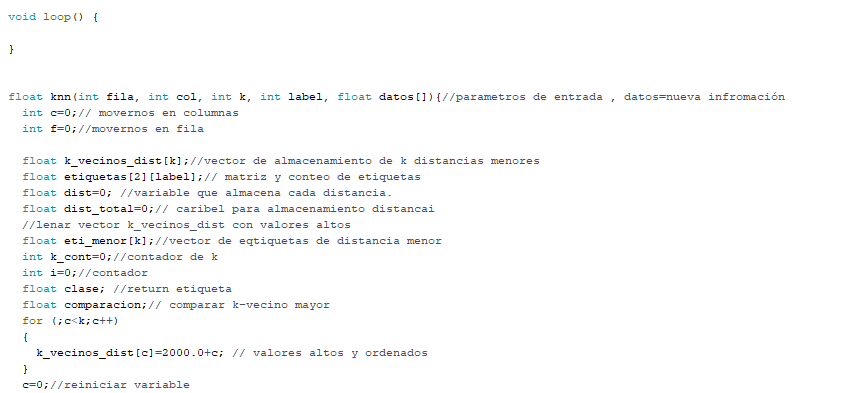
\includegraphics[scale=0.9]{c12.png}
\end{figure}

\begin{figure}[H]
\caption{Código Parte 13}
\centering
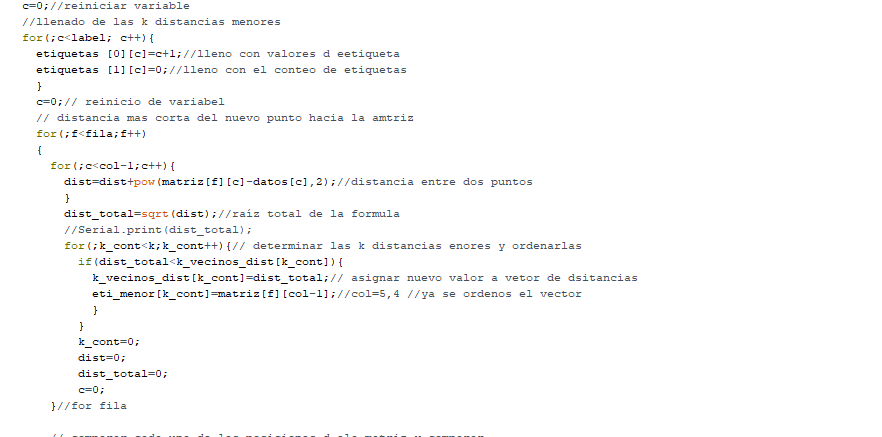
\includegraphics[scale=0.9]{c13.png}
\end{figure}

\begin{figure}[H]
\caption{Código Parte 14}
\centering
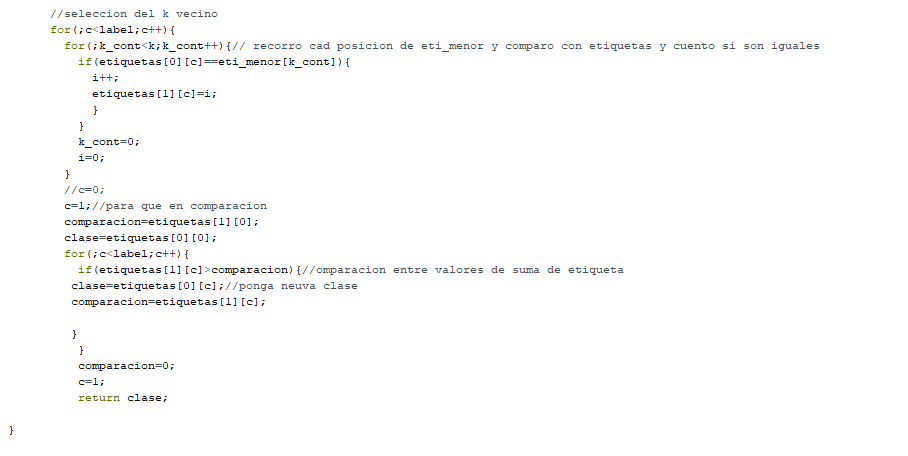
\includegraphics[scale=0.9]{c14.png}
\end{figure}

\begin{figure}[H]
\caption{Código Parte 15}
\centering
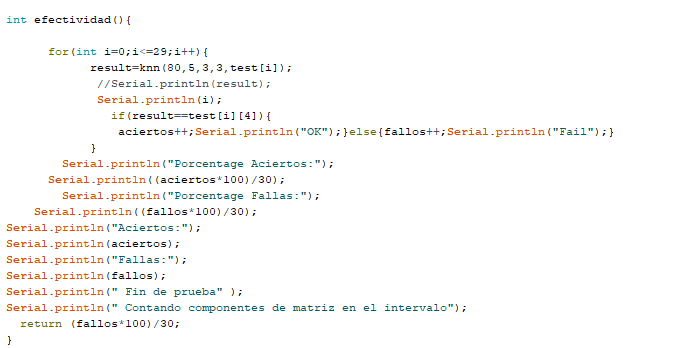
\includegraphics[scale=0.9]{c15.png}
\end{figure}
\\
Al final se obtiene la siguiente matriz la cual en este caso va a ser la de mejor resultado en las donas, la cual en este caso esta compuesta de [9][5].
\begin{figure}[H]
\caption{Resultado de Matriz Final}
\centering
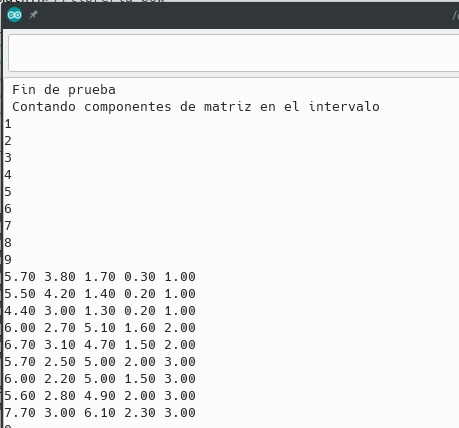
\includegraphics[scale=0.9]{matrizfinal.jpg}
\end{figure}
\\
Finalmente tenemos nuestra tabla de eficiencia la cual muestra el porcentaje de eficiencia de cada dona y selecciona la mejor para guardarla mostrarla y generar de esta forma la mejor matriz de comparacion.
\begin{figure}[H]
\caption{Tabla de Resultados en Eficiencia}
\centering
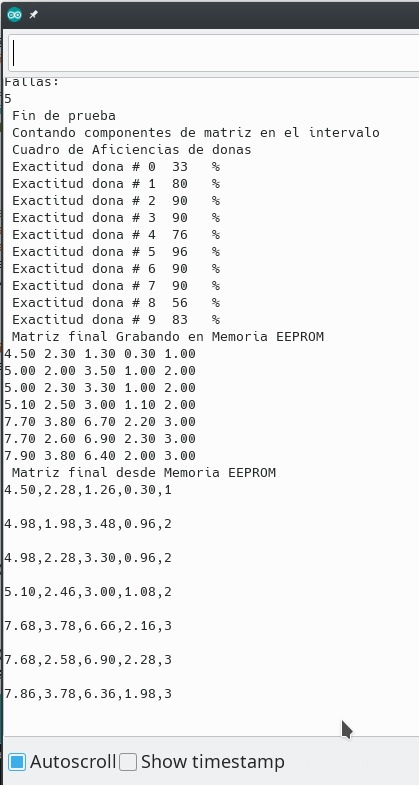
\includegraphics[scale=0.9]{tablaefi.jpg}
\end{figure}
\\
\section{Conclusiones y Recomendaciones}
\subsection{Conclusiones}
- El método de donas nos ayuda a poder excluir datos que no son necesarios eso sí se debe escoger la que 	mejor eficiencia presente al momento de comparar valores de prueba. El algoritmo de KNN es de mucha importancia para la realización de este proyecto ya que de esto depende el algoritmo de CNN para poder clasificar qué métodos van a la matriz S o la matriz D.\\
- El algoritmo que se ha desarrollado con cnn y knn es modular ya que puede ser ampliado a cuantas variables o tipos de datos a clasificar.\\
- Mientras más variables el algoritmo tiene que analizar muchos más recursos utilizara para ju ejecución lo que podría limitar el desarrollo y normal operación del mismo en grandes cantidades de información.\\
\subsection{Recomendaciones}
- Comprobar antes de realizar demasiado código que lo que estamos realizando funcione de manera correcta para que en caso de que haya algún error sea fácil de solucionar.\\
- Escoger los mejores datos para que al momento de comprobar los datos de prueba se obtenga una buena eficiencia es decir muchos más aciertos que errores.\\
- Limitar el numero de variables a utilizar debido a la poca capacidad de procesamiento que nos brinda nuestra plataforma arduino.\\
- Comentar el código para de esta manera sea mucho mas fácil su modificación y adaptación.\\
\end{document}